\section{Implementation}
%%%%%%%%%%%% MID WAY AGENDA %%%%%%%%%%%%%%
%\begin{frame}<beamer>
%\frametitle{Thomas Holm Pilgaard}
%\tableofcontents[currentsection]
%\end{frame}
%%%%%%%%%%%% MID WAY AGENDA %%%%%%%%%%%%%%

% \begin{frame}{Parameter identification results}{Wrong measurement data}

% \begin{itemize}
% 	 	\item<1-> Measurement data is not around the operating point
% 	 	\item<1-> Steady state error in the model
% 	 	\end{itemize}

% \begin{figure}[H]
%    \centering
%     \input{Tikz/WT_figure.tex}
% \end{figure}

% \begin{figure}[H]
%    \centering
%     \input{Tikz/WT_figure1.tex}
% \end{figure}

% \end{frame}

\begin{frame}{Implementation method}{Simulink}
\begin{itemize}
\item<1-> MPC control strategy for 24 hours
\item<1-> At each hour:
	 	\begin{itemize}
	 	\item<1-> Iterate $\hat{\pmb{d}}[k]$ and $c_p [k]$
	 	\item<1-> Measurement on the states 
	 	\item<1-> Apply control input $\pmb{\hat{u}_{Hp}}(1,1)$
	 	\end{itemize}
\end{itemize}

\begin{figure}[H]
\centering
\input{Tikz/Control_Layout.tex} 
\end{figure}

\end{frame}


\subsection{Implementation results}

\begin{frame}{Implementation results}{For one iteration}

\begin{itemize}
	 	\item<1-> Softened constraints on $\hat{\pmb{\underline{u}}}_{Hp}$
	 	\end{itemize}

\begin{figure}[H]
   \centering
    % This file was created by matlab2tikz.
%
%The latest updates can be retrieved from
%  http://www.mathworks.com/matlabcentral/fileexchange/22022-matlab2tikz-matlab2tikz
%where you can also make suggestions and rate matlab2tikz.
%
\definecolor{mycolor1}{rgb}{0.00000,0.44700,0.74100}%
%
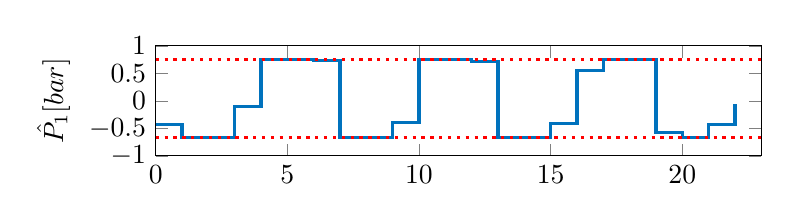
\begin{tikzpicture}

\begin{axis}[%
width=3.028in,
height=0.55in,at={(1.011in,4.137in)},
scale only axis,
xmin=0,
xmax=23,
ymin=-1,
ymax=1,
ylabel={$\hat{P_1}[bar]$},
%xmajorgrids,
%ymajorgrids,
axis background/.style={fill=white},
title style={font=\bfseries},
%title={$\text{u}_{\text{hp1}}\text{[k=0]}$}
]
\addplot[const plot,color=mycolor1,solid,forget plot,very thick] plot table[row sep=crcr] {%
0	-0.433446931217239\\
1	-0.669999999998947\\
2	-0.669999999997713\\
3	-0.104236955958482\\
4	0.749999999997401\\
5	0.749999999998619\\
6	0.727077455814283\\
7	-0.669999999999055\\
8	-0.66999999999925\\
9	-0.395725243988171\\
10	0.749999999988271\\
11	0.749999999998319\\
12	0.717572940373614\\
13	-0.669999999998221\\
14	-0.669999999999149\\
15	-0.409583761852645\\
16	0.548034702463677\\
17	0.749999999998184\\
18	0.74999999999883\\
19	-0.576396407197271\\
20	-0.669999999998877\\
21	-0.425048538821507\\
22	-0.0640667111129486\\
};
\addplot[const plot,color=red,dotted,very thick] plot table[row sep=crcr] {%
0	0.75\\
24	0.75\\
};

\addplot[const plot,color=red,dotted,very thick] plot table[row sep=crcr] {%
0	-0.67\\
24	-0.67\\
};

\end{axis}
\end{tikzpicture}


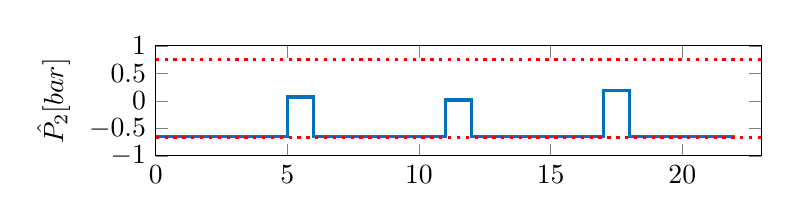
\begin{tikzpicture}

\begin{axis}[%
width=3.028in,
height=0.55in,
at={(1.011in,2.39in)},
scale only axis,
xmin=0,
xmax=23,
ymin=-1,
ymax=1,
%xmajorgrids,
%ymajorgrids,
ylabel={$\hat{P_2}[bar]$},
axis background/.style={fill=white},
title style={font=\bfseries},
%title={$\text{u}_{\text{hp2}}\text{[k=0]}$}
]
\addplot[const plot,color=mycolor1,solid,forget plot,very thick] plot table[row sep=crcr] {%
0	-0.649999999999008\\
1	-0.649999999999539\\
2	-0.649999999999527\\
3	-0.64999999999887\\
4	-0.649999999994262\\
5	0.0667700518106753\\
6	-0.649999999998485\\
7	-0.649999999999511\\
8	-0.649999999999588\\
9	-0.649999999999157\\
10	-0.649999999997306\\
11	0.0160826405819198\\
12	-0.649999999996155\\
13	-0.64999999999941\\
14	-0.64999999999958\\
15	-0.649999999999219\\
16	-0.649999999998156\\
17	0.189015571020597\\
18	-0.649999999956971\\
19	-0.649999999999335\\
20	-0.649999999999555\\
21	-0.649999999999218\\
22	-0.649999999998207\\
};
\addplot[const plot,color=red,dotted,very thick] plot table[row sep=crcr] {%
0	0.75\\
24	0.75\\
};

\addplot[const plot,color=red,dotted,very thick] plot table[row sep=crcr] {%
0	-0.67\\
24	-0.67\\
};
\end{axis}
\end{tikzpicture}

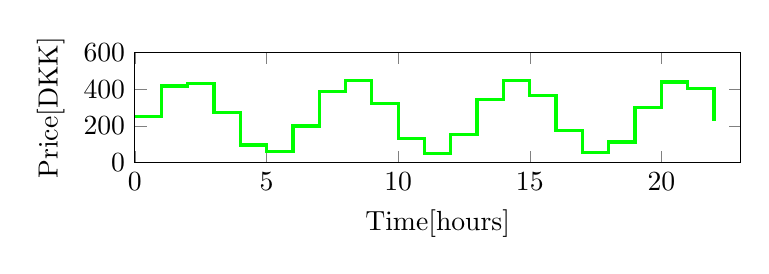
\begin{tikzpicture}

\begin{axis}[%
width=3.028in,
height=0.55in,
at={(1.011in,0.642in)},
scale only axis,
xmin=0,
xmax=23,
xlabel={Time[hours]},
ymin=0,
ymax=600,
%xmajorgrids,
%ymajorgrids,
ylabel={Price[DKK]},
axis background/.style={fill=white},
title style={font=\bfseries},
]
\addplot[const plot,color=green,solid,forget plot,very thick] plot table[row sep=crcr] {%
0	250\\
1	418.857649358291\\
2	430.978019589665\\
3	275.110723996831\\
4	95.9351176989303\\
5	59.7658279797972\\
6	200.175962602534\\
7	386.833833626164\\
8	446.479615730073\\
9	323.748819156816\\
10	132.562792409559\\
11	50.3844917318038\\
12	153.493572208496\\
13	346.181981592006\\
14	449.592219965457\\
15	367.736693884804\\
16	176.595452155304\\
17	53.5898806097876\\
18	112.896379753435\\
19	299.465389524004\\
20	440.119567515206\\
21	404.300699515516\\
22	225.256624358491\\
};
\end{axis}
\end{tikzpicture}%
\end{figure}

\end{frame}


\section{Discussion}
\begin{frame}{Discussion}{}

\begin{itemize}
	\item<1-> Possible improvements and error fixing
	\begin{itemize}
	 \item<1-> Long measurements, ensuring initial steady state condition
	 \item<1-> Correcting the implementation
	 \item<1-> Different softened constraint configurations

	\end{itemize}
\end{itemize}

\begin{itemize}
\item<2-> Considerations for future work
	 \begin{itemize}
	 \item<2-> Using the end-user pressure measurements
	 \item<2-> Robust MPC
	 \item<2-> Non-linear model fixing

		\begin{itemize}
	 	\item<3-> Online linearization
	 	\item<3-> Operating points are constantly varied
	 	\item<3-> Precision is more reliable
	 	\end{itemize}

	 \end{itemize}
\end{itemize}

\end{frame}
